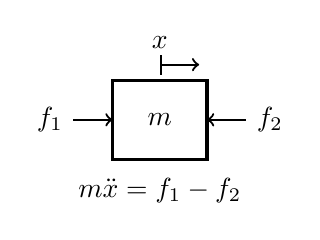
\begin{tikzpicture}
    \draw[very thick] (0,0) rectangle (1.2,1);
    \draw (.6,.5) node {$m$};
    \draw[<-,thick] (1.2,.5) -- ++(.5,0) node[right] {$f_{2}$};
    \draw[<-,thick] (0,.5) -- ++(-.5,0) node[left] {$f_{1}$};
    \draw[|->,thick] (.6,1.2) node[above=2pt] {$x$} -- ++(.5,0);  
        \draw<2-> (.6,-.4) node {$m\ddot{x}=f_{1}-f_{2}$};

\end{tikzpicture}
